%============================================================
%  Chapter 3 — Technical Study
%============================================================
\chapter{Technical Study}
\label{chap:technical}

\section{Introduction}

This chapter provides the most detailed technical exposition of the Vulnerability Management System. We present the technology stack selection rationale, the three-tier architecture, the complete 10-table database schema, key algorithms and data flows, and the integration designs for both Tenable Nessus and Ollama LLM.

\section{Technology Stack}

\begin{figure}[H]
\centering
\begin{tikzpicture}
\def\tech#1#2#3{
  \node[draw=#3!60, fill=#3!10, rounded corners=4pt, minimum width=2.6cm,
        minimum height=1.1cm, font=\bfseries\small, text=#3!80!black,
        align=center] {#1\\{\tiny #2}};
}
\matrix[column sep=0.5cm, row sep=0.4cm]{
  \tech{Python 3.11}{Backend Language}{ISIblue} &
  \tech{Flask 3.0}{Web Framework}{ISIblue} &
  \tech{SQLAlchemy}{ORM}{ISIblue} &
  \tech{PostgreSQL 16}{Database}{ISIblue} \\
  \tech{Ollama}{LLM Runtime}{orange} &
  \tech{Mistral 7B}{AI Model}{orange} &
  \tech{Tenable API}{Scanner Integration}{critical} &
  \tech{Jinja2}{Template Engine}{low} \\
  \tech{Bootstrap 5}{CSS Framework}{ISIblue!60} &
  \tech{Docker}{Containerization}{ISIblue!80} &
  \tech{Flask-Mail}{SMTP Email}{low} &
  \tech{bcrypt}{Password Hashing}{critical} \\
};
\end{tikzpicture}
\caption{VMS Technology Stack}
\label{fig:techstack}
\end{figure}

\subsection{Backend: Python and Flask}

Python 3.11 was chosen as the primary programming language for its rich ecosystem of security and data processing libraries, rapid development capabilities, and strong community support. Flask~\cite{flask2024} provides a lightweight, unopinionated web framework that gives full control over application structure while offering essential extensions.

Key Flask extensions used:
\begin{itemize}
  \item \textbf{Flask-SQLAlchemy}: ORM integration for database access
  \item \textbf{Flask-Login}: Session management and authentication
  \item \textbf{Flask-Mail}: Email notification delivery via SMTP
  \item \textbf{Flask-WTF}: Form handling and CSRF protection
  \item \textbf{Flask-Migrate}: Database schema migration management
\end{itemize}

\subsection{Database: PostgreSQL}

PostgreSQL 16~\cite{postgresql2024} was selected over alternatives (MySQL, SQLite) for its superior support for complex queries, full ACID compliance, advanced indexing strategies, and JSON data type support. The vulnerability data ingested from Nessus contains nested JSON structures that benefit from PostgreSQL's native JSON/JSONB support.

\subsection{AI Integration: Ollama with Mistral 7B}

The most distinctive technical choice in this project is the use of Ollama~\cite{ollama2024} for local LLM deployment. Ollama is an open-source runtime that enables running large language models entirely on local hardware through a simple REST API.

\begin{keybox}
\textbf{Why Ollama Over Cloud APIs?}

During initial prototyping, the Claude API (claude-haiku) was tested for remediation suggestions. While effective, this approach raised a fundamental concern: vulnerability details — including CVE identifiers, affected asset IP addresses, open ports, and organizational context — were being transmitted to external cloud servers. This is unacceptable for security-sensitive applications. The migration to Ollama/Mistral 7B eliminates this risk entirely. All AI inference runs on the local server, and no data ever leaves the organization's network.
\end{keybox}

The Mistral 7B model~\cite{mistral2024} offers an excellent balance of instruction-following capability and hardware requirements (runs on 8GB RAM with CPU inference, or faster with GPU).

\section{Three-Tier Architecture}

\begin{figure}[H]
\centering
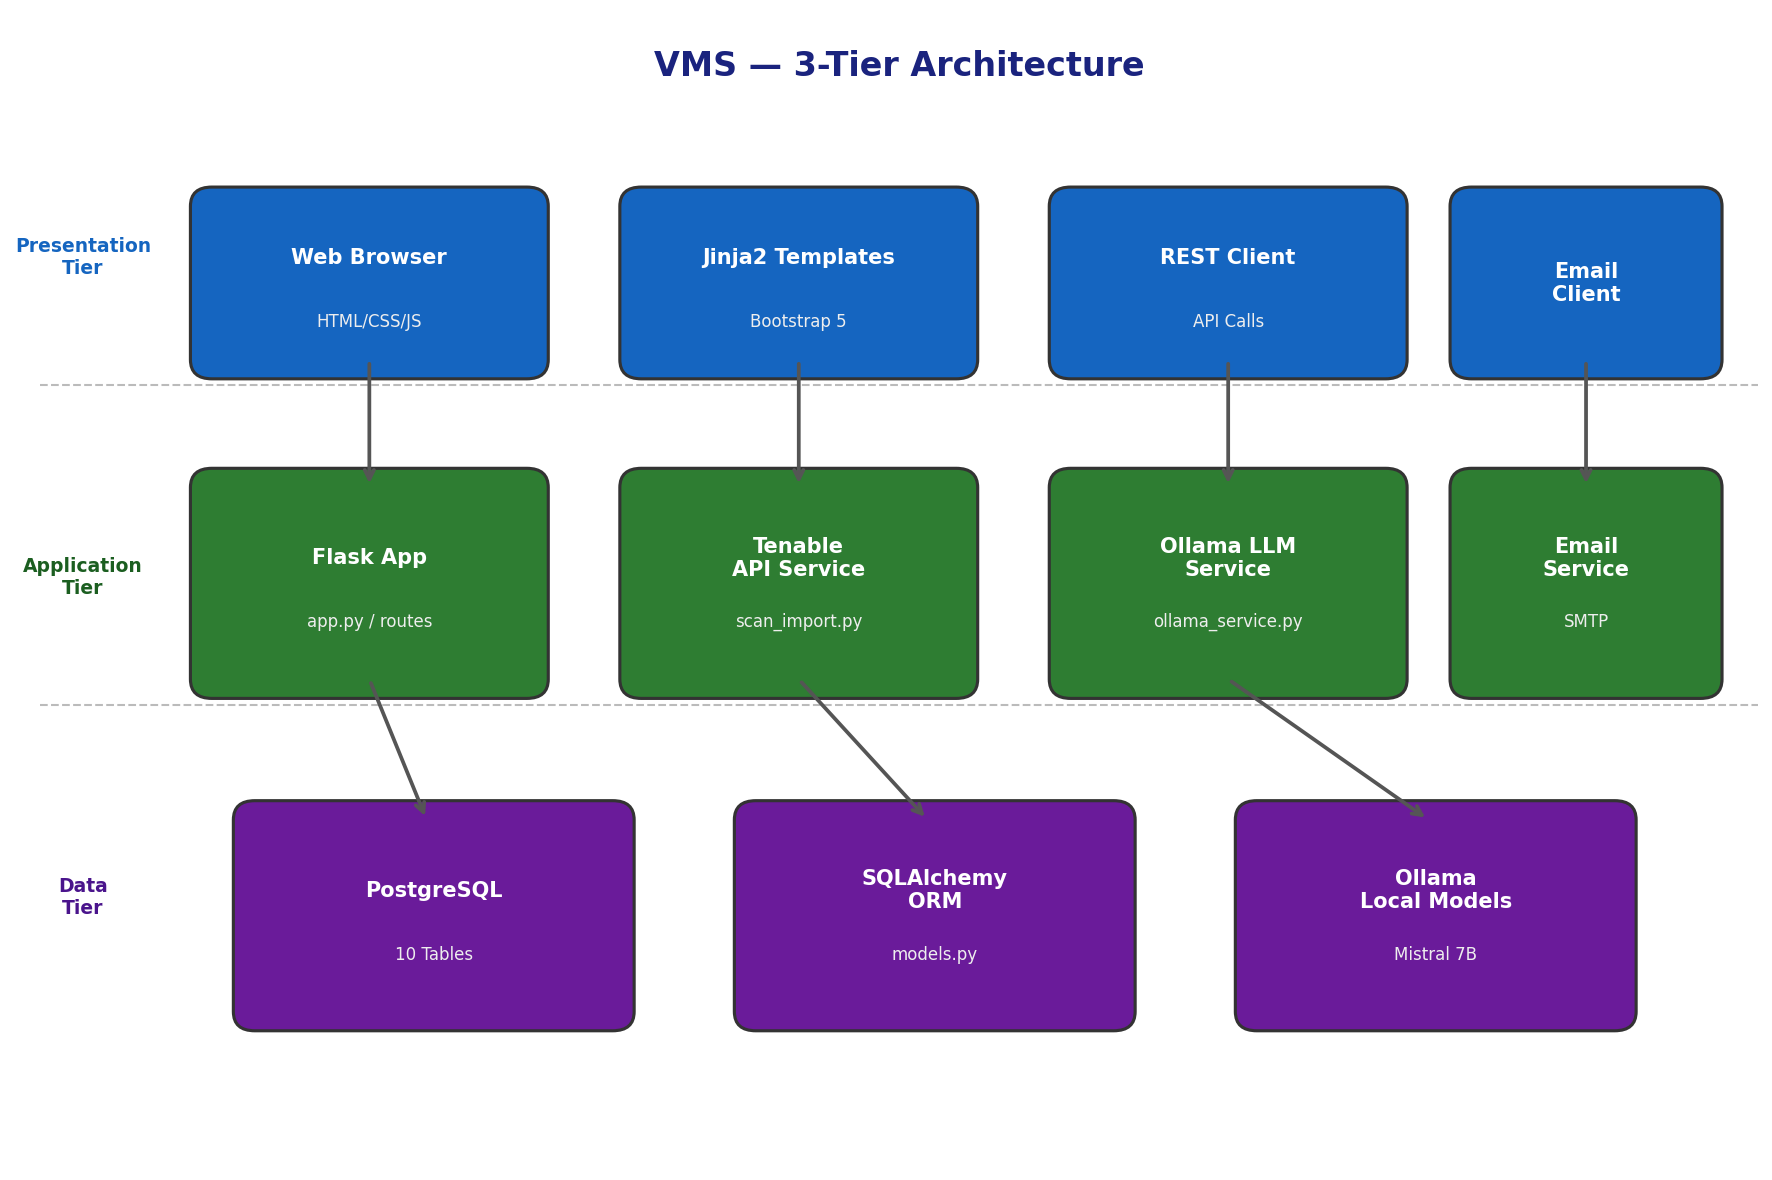
\includegraphics[width=0.95\linewidth]{img/architecture.png}
\caption{VMS Three-Tier Architecture}
\label{fig:architecture}
\end{figure}

The VMS follows a classic three-tier architecture separating presentation, application logic, and data persistence:

\subsection{Presentation Tier}
The presentation tier consists of Jinja2-rendered HTML templates styled with Bootstrap 5. The frontend is deliberately server-rendered to minimize JavaScript complexity and ensure functionality without modern JS frameworks. Key pages include:

\begin{itemize}
  \item \textbf{Dashboard}: KPI cards, severity charts, overdue findings table
  \item \textbf{Findings List}: Filterable, sortable table with severity badges and status indicators
  \item \textbf{Finding Detail}: Full vulnerability details, status update form, Ollama chat interface
  \item \textbf{Risk Acceptances}: Pending requests list for managers
  \item \textbf{Admin Panel}: User management, SLA configuration, asset registry
\end{itemize}

\subsection{Application Tier}
The Flask application handles routing, business logic, and service orchestration. The application is organized into logical modules:

\begin{lstlisting}[style=python, caption={Application Module Structure}, label={lst:structure}]
vms/
├── app.py                 # Application factory and route handlers
├── models.py              # SQLAlchemy model definitions (10 tables)
├── services/
│   ├── scan_import.py     # Tenable Nessus API integration
│   ├── ollama_service.py  # Ollama LLM chat interface
│   ├── email_service.py   # Email notification delivery
│   ├── sla_service.py     # SLA calculation and overdue detection
│   └── risk_service.py    # Risk acceptance workflow
├── templates/             # Jinja2 HTML templates
│   ├── base.html
│   ├── dashboard.html
│   ├── findings/
│   └── admin/
└── static/                # CSS, JS, images
\end{lstlisting}

\subsection{Data Tier}
The data tier consists of a PostgreSQL database accessed exclusively through SQLAlchemy ORM. Ollama models are stored locally in the \texttt{/root/.ollama/models} directory on the application server.

\section{Component Diagram}

\begin{figure}[H]
\centering
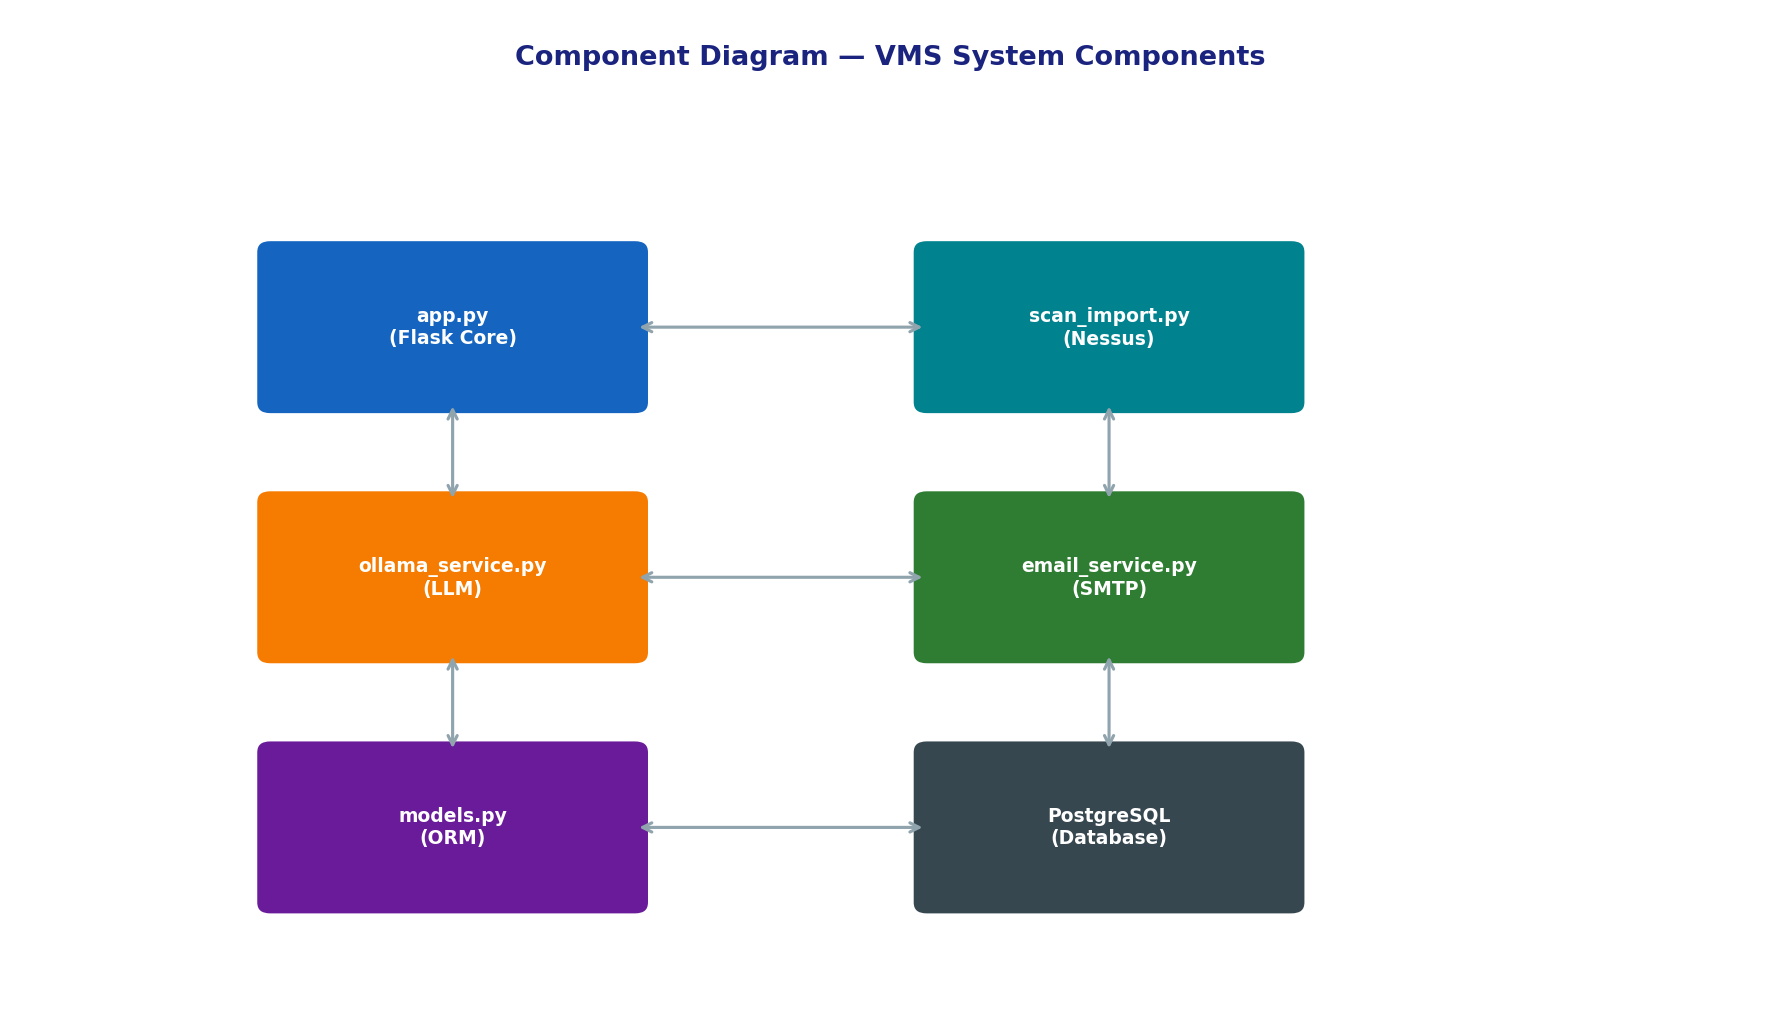
\includegraphics[width=0.88\linewidth]{img/components.png}
\caption{VMS Component Diagram}
\label{fig:components}
\end{figure}

\section{Database Schema — 10 Tables}

\begin{figure}[H]
\centering
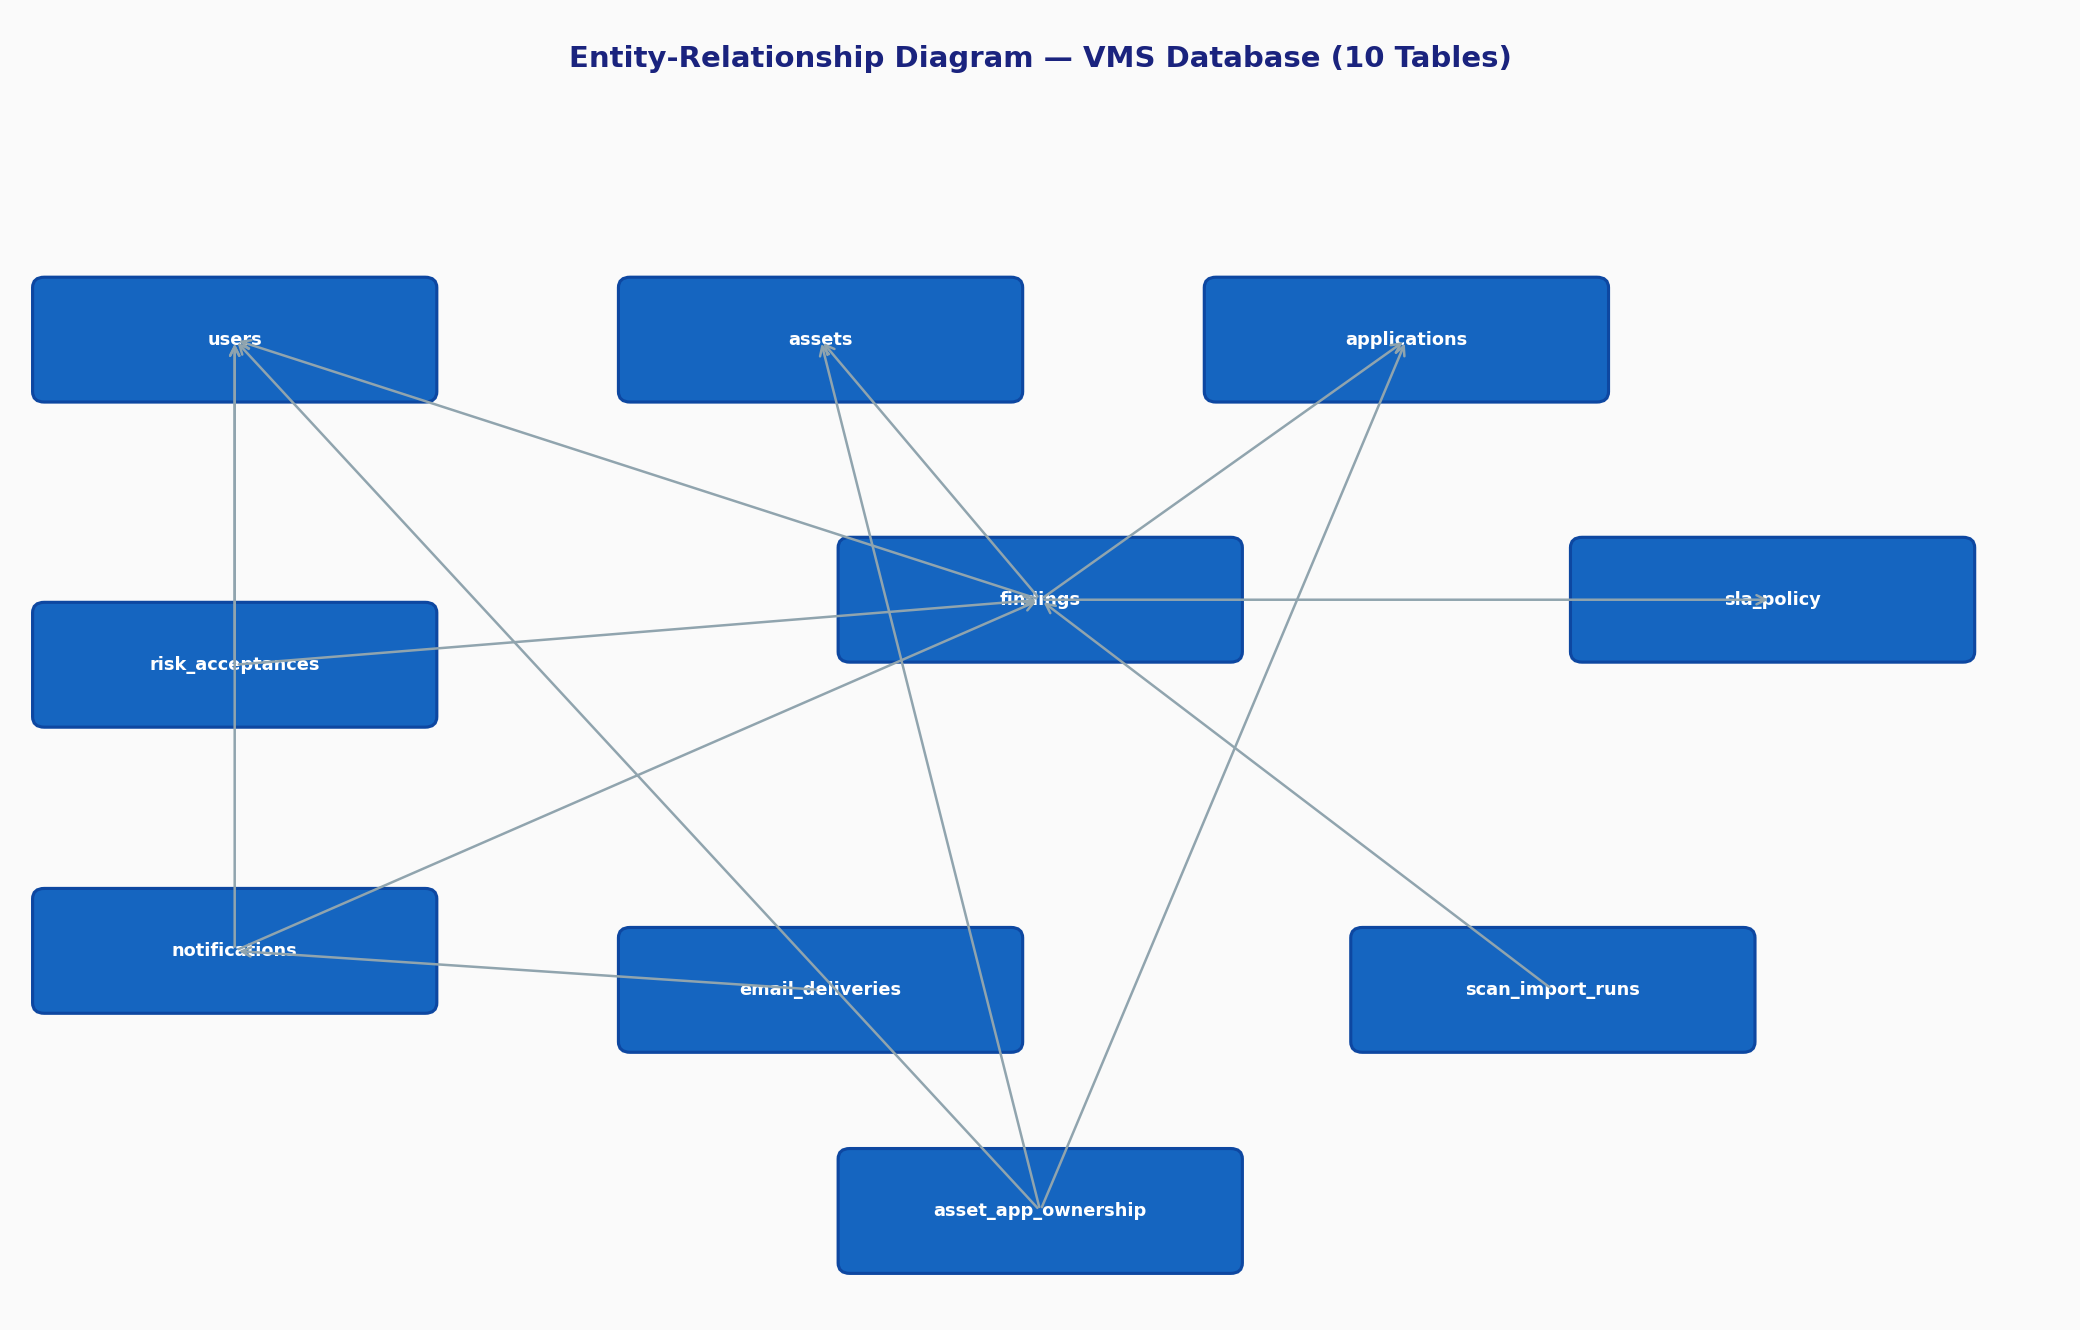
\includegraphics[width=0.95\linewidth]{img/erd.png}
\caption{Entity-Relationship Diagram — VMS Database}
\label{fig:erd}
\end{figure}

\subsection{Table Definitions}

\subsubsection{users}
Stores all authenticated users of the VMS application.

\begin{lstlisting}[style=sql, caption={users table DDL}, label={lst:users}]
CREATE TABLE users (
    id          SERIAL PRIMARY KEY,
    username    VARCHAR(80)  UNIQUE NOT NULL,
    email       VARCHAR(120) UNIQUE NOT NULL,
    password    VARCHAR(256) NOT NULL,       -- bcrypt hash
    role        VARCHAR(30)  NOT NULL        -- analyst|sysadmin|manager|admin
                CHECK (role IN ('analyst','sysadmin','manager','admin')),
    is_active   BOOLEAN DEFAULT TRUE,
    created_at  TIMESTAMP DEFAULT NOW(),
    last_login  TIMESTAMP
);
\end{lstlisting}

\subsubsection{assets}
Represents network-connected hosts scanned by Nessus.

\begin{lstlisting}[style=sql, caption={assets table DDL}, label={lst:assets}]
CREATE TABLE assets (
    id          SERIAL PRIMARY KEY,
    ip_address  INET NOT NULL UNIQUE,
    hostname    VARCHAR(255),
    os          VARCHAR(120),
    asset_type  VARCHAR(50),    -- server|workstation|network_device|vm
    description TEXT,
    owner_id    INTEGER REFERENCES users(id),
    created_at  TIMESTAMP DEFAULT NOW(),
    updated_at  TIMESTAMP DEFAULT NOW()
);
\end{lstlisting}

\subsubsection{applications}
Represents software applications or services mapped to assets.

\begin{lstlisting}[style=sql, caption={applications table DDL}, label={lst:apps}]
CREATE TABLE applications (
    id          SERIAL PRIMARY KEY,
    name        VARCHAR(150) NOT NULL,
    description TEXT,
    version     VARCHAR(50),
    env         VARCHAR(30)  -- dev|staging|production
                CHECK (env IN ('dev','staging','production')),
    owner_id    INTEGER REFERENCES users(id),
    created_at  TIMESTAMP DEFAULT NOW()
);
\end{lstlisting}

\subsubsection{findings}
The central table of the VMS, representing individual vulnerability findings.

\begin{lstlisting}[style=sql, caption={findings table DDL}, label={lst:findings}]
CREATE TABLE findings (
    id              SERIAL PRIMARY KEY,
    asset_id        INTEGER NOT NULL REFERENCES assets(id),
    application_id  INTEGER REFERENCES applications(id),
    plugin_id       INTEGER NOT NULL,
    plugin_name     VARCHAR(500) NOT NULL,
    severity        VARCHAR(20) NOT NULL
                    CHECK (severity IN ('Critical','High','Medium','Low','Info')),
    cvss_score      NUMERIC(4,1),
    cve_ids         TEXT[],            -- Array of CVE identifiers
    description     TEXT,
    solution        TEXT,
    port            INTEGER DEFAULT 0,
    protocol        VARCHAR(10) DEFAULT '/',
    status          VARCHAR(30) NOT NULL DEFAULT 'NEW'
                    CHECK (status IN ('NEW','ASSIGNED','IN_PROGRESS',
                                      'REMEDIATED','VERIFIED','CLOSED',
                                      'FALSE_POSITIVE','ACCEPTED_RISK')),
    assigned_to_id  INTEGER REFERENCES users(id),
    due_date        TIMESTAMP,
    first_seen      TIMESTAMP NOT NULL DEFAULT NOW(),
    last_seen       TIMESTAMP NOT NULL DEFAULT NOW(),
    remediation_note TEXT,
    UNIQUE (asset_id, plugin_id, port, protocol)  -- Deduplication key
);

CREATE INDEX idx_findings_severity ON findings(severity);
CREATE INDEX idx_findings_status   ON findings(status);
CREATE INDEX idx_findings_due_date ON findings(due_date);
CREATE INDEX idx_findings_asset_id ON findings(asset_id);
\end{lstlisting}

\subsubsection{risk\_acceptances}
Manages the formal risk acceptance approval workflow.

\begin{lstlisting}[style=sql, caption={risk\_acceptances table DDL}, label={lst:risk}]
CREATE TABLE risk_acceptances (
    id              SERIAL PRIMARY KEY,
    finding_id      INTEGER NOT NULL REFERENCES findings(id),
    requested_by_id INTEGER NOT NULL REFERENCES users(id),
    reviewed_by_id  INTEGER REFERENCES users(id),
    status          VARCHAR(20) NOT NULL DEFAULT 'PENDING'
                    CHECK (status IN ('PENDING','APPROVED','REJECTED')),
    justification   TEXT NOT NULL,
    review_note     TEXT,
    requested_at    TIMESTAMP DEFAULT NOW(),
    reviewed_at     TIMESTAMP
);
\end{lstlisting}

\subsubsection{sla\_policy}
Configurable SLA definitions by severity level.

\begin{lstlisting}[style=sql, caption={sla\_policy table DDL}, label={lst:sla}]
CREATE TABLE sla_policy (
    id              SERIAL PRIMARY KEY,
    severity        VARCHAR(20) UNIQUE NOT NULL,
    days_to_fix     INTEGER NOT NULL,  -- Calendar days for remediation
    warn_at_percent INTEGER DEFAULT 50, -- % elapsed before warning email
    is_active       BOOLEAN DEFAULT TRUE,
    updated_at      TIMESTAMP DEFAULT NOW()
);

INSERT INTO sla_policy (severity, days_to_fix) VALUES
  ('Critical', 7), ('High', 15), ('Medium', 30), ('Low', 60);
\end{lstlisting}

\subsubsection{notifications}
Log of all notification events generated by the system.

\begin{lstlisting}[style=sql, caption={notifications table DDL}, label={lst:notif}]
CREATE TABLE notifications (
    id              SERIAL PRIMARY KEY,
    finding_id      INTEGER REFERENCES findings(id),
    recipient_id    INTEGER REFERENCES users(id),
    type            VARCHAR(30) NOT NULL
                    CHECK (type IN ('ASSIGNED','OVERDUE','HALF_SLA',
                                    'UNMAPPED_FINDINGS','RISK_ACCEPTANCE_REQUEST')),
    message         TEXT,
    created_at      TIMESTAMP DEFAULT NOW(),
    is_read         BOOLEAN DEFAULT FALSE
);
\end{lstlisting}

\subsubsection{email\_deliveries}
Tracks email notification delivery for audit and retry purposes.

\begin{lstlisting}[style=sql, caption={email\_deliveries table DDL}, label={lst:email}]
CREATE TABLE email_deliveries (
    id              SERIAL PRIMARY KEY,
    notification_id INTEGER NOT NULL REFERENCES notifications(id),
    recipient_email VARCHAR(120) NOT NULL,
    subject         VARCHAR(250),
    status          VARCHAR(20) DEFAULT 'PENDING'
                    CHECK (status IN ('PENDING','SENT','FAILED')),
    sent_at         TIMESTAMP,
    error_message   TEXT,
    retry_count     INTEGER DEFAULT 0
);
\end{lstlisting}

\subsubsection{scan\_import\_runs}
Audit log of every Nessus scan import operation.

\begin{lstlisting}[style=sql, caption={scan\_import\_runs table DDL}, label={lst:scanimport}]
CREATE TABLE scan_import_runs (
    id              SERIAL PRIMARY KEY,
    triggered_by_id INTEGER REFERENCES users(id),
    status          VARCHAR(20) DEFAULT 'RUNNING'
                    CHECK (status IN ('RUNNING','SUCCESS','FAILED')),
    total_fetched   INTEGER DEFAULT 0,
    new_findings    INTEGER DEFAULT 0,
    updated_findings INTEGER DEFAULT 0,
    error_message   TEXT,
    started_at      TIMESTAMP DEFAULT NOW(),
    completed_at    TIMESTAMP
);
\end{lstlisting}

\subsubsection{asset\_app\_ownership}
Junction table mapping assets to applications and their owners.

\begin{lstlisting}[style=sql, caption={asset\_app\_ownership table DDL}, label={lst:ownership}]
CREATE TABLE asset_app_ownership (
    id              SERIAL PRIMARY KEY,
    asset_id        INTEGER NOT NULL REFERENCES assets(id),
    application_id  INTEGER NOT NULL REFERENCES applications(id),
    owner_id        INTEGER NOT NULL REFERENCES users(id),
    assigned_at     TIMESTAMP DEFAULT NOW(),
    UNIQUE (asset_id, application_id)
);
\end{lstlisting}

\section{Key Algorithms and Data Flows}

\subsection{Vulnerability Management Lifecycle}

\begin{figure}[H]
\centering
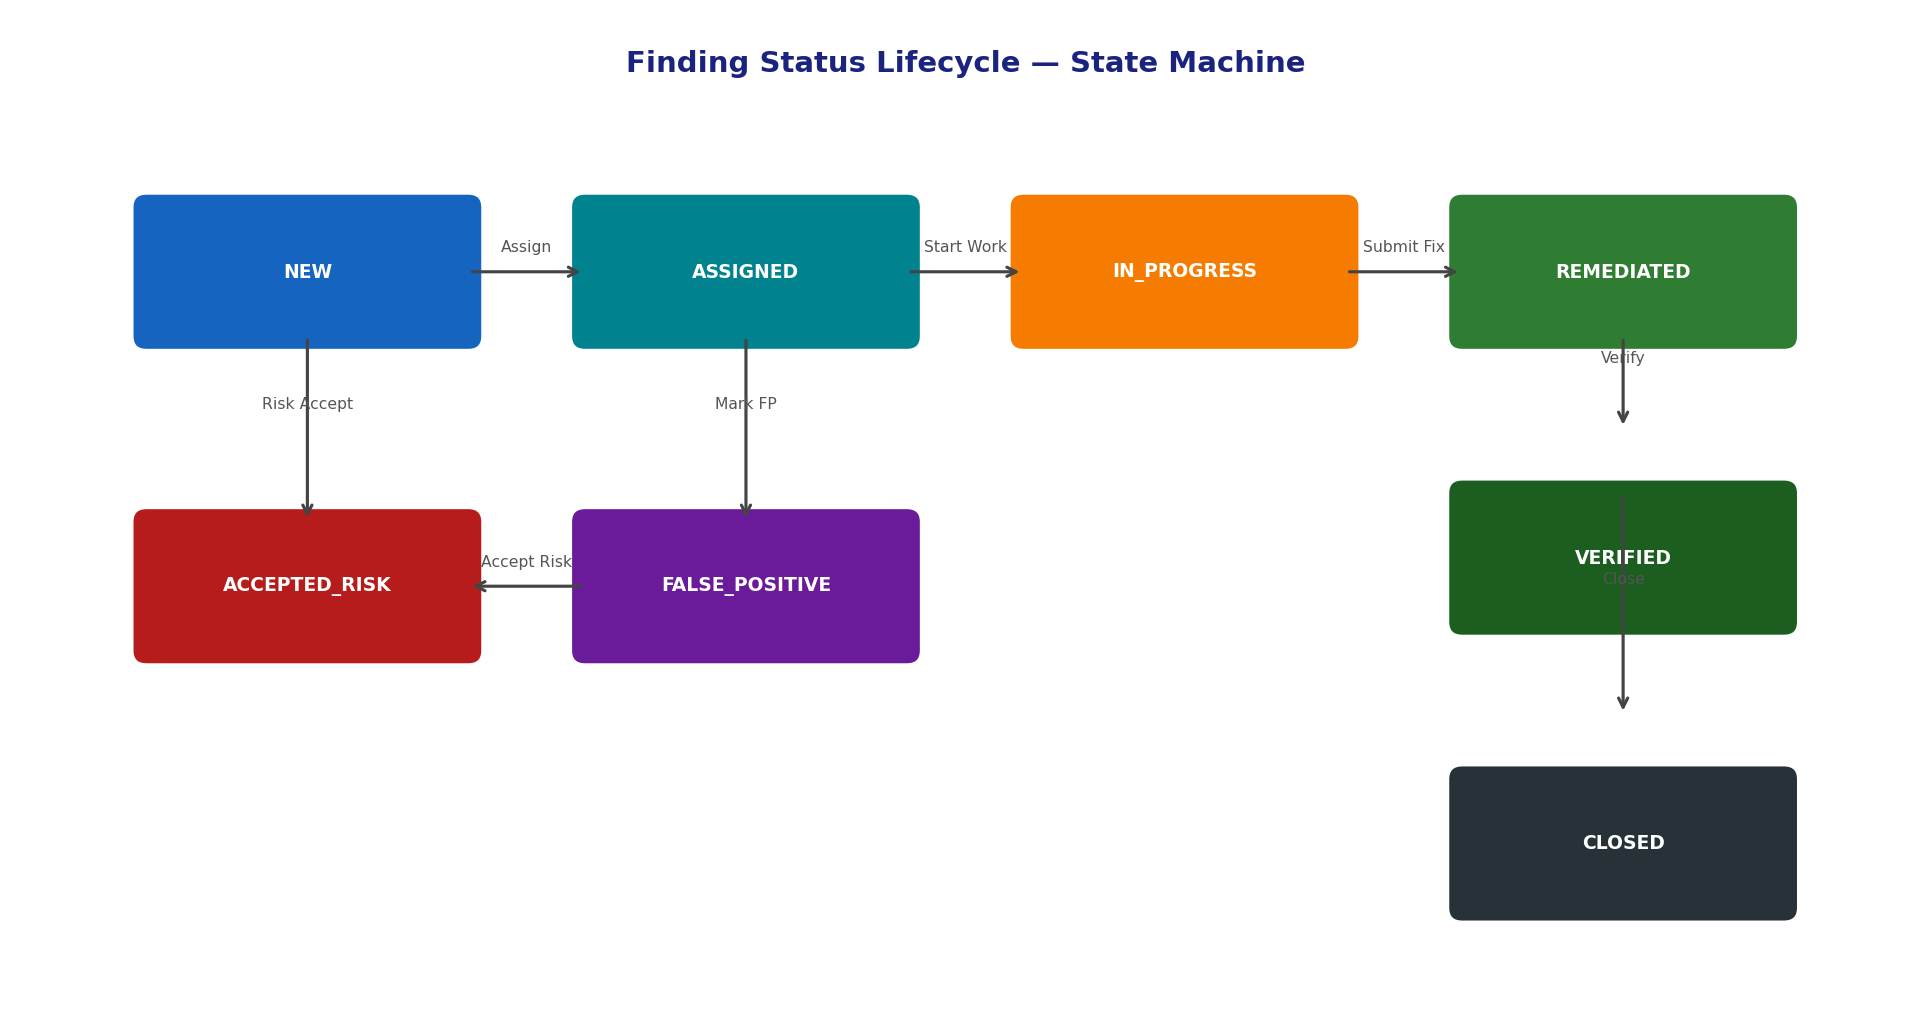
\includegraphics[width=0.95\linewidth]{img/statemachine.png}
\caption{Finding Status State Machine}
\label{fig:statemachine}
\end{figure}

The finding lifecycle follows a state machine with the following transitions:

\begin{table}[H]
\centering
\caption{Valid Finding Status Transitions}
\label{tab:transitions}
\begin{tabular}{lll}
\toprule
\textbf{From} & \textbf{To} & \textbf{Trigger} \\
\midrule
NEW & ASSIGNED & Analyst assigns to Sysadmin \\
NEW & FALSE\_POSITIVE & Analyst marks as FP \\
ASSIGNED & IN\_PROGRESS & Sysadmin starts remediation \\
IN\_PROGRESS & REMEDIATED & Sysadmin submits fix \\
IN\_PROGRESS & ACCEPTED\_RISK & Manager approves risk acceptance \\
REMEDIATED & VERIFIED & Analyst confirms fix after re-scan \\
VERIFIED & CLOSED & Analyst closes the finding \\
CLOSED & NEW & Re-detected in subsequent scan \\
\bottomrule
\end{tabular}
\end{table}

\subsection{Scan Import Flow}

\begin{figure}[H]
\centering
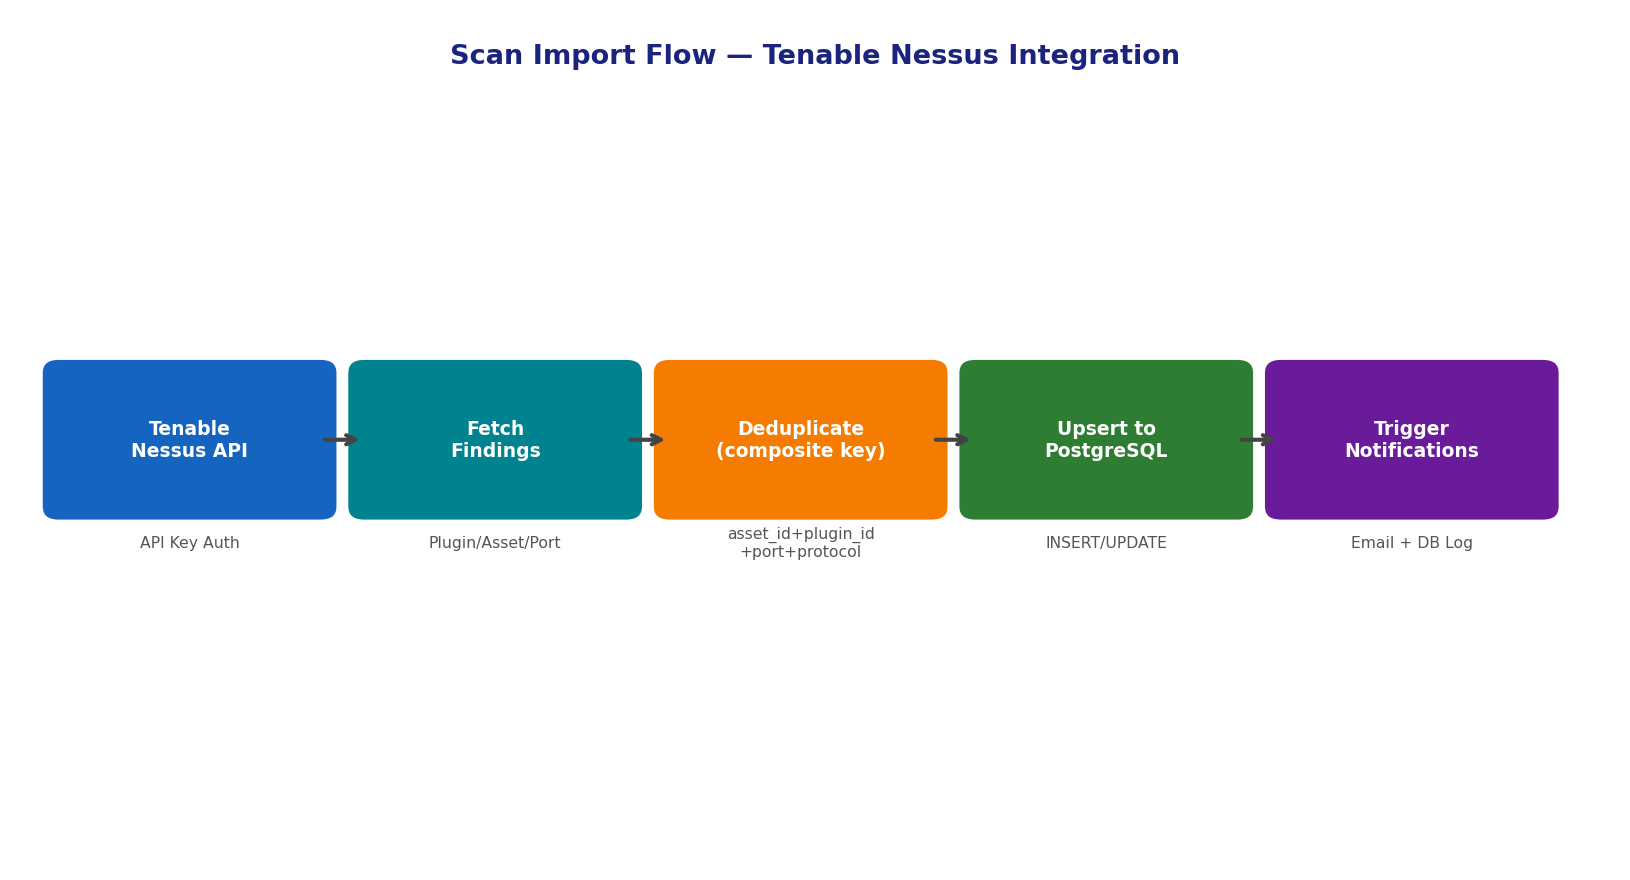
\includegraphics[width=0.92\linewidth]{img/importflow.png}
\caption{Tenable Nessus Scan Import Flow}
\label{fig:importflow}
\end{figure}

\begin{lstlisting}[style=python, caption={Scan Import Core Logic}, label={lst:import}]
def import_nessus_findings(run_id: int) -> dict:
    """
    Fetch findings from Tenable API and upsert into database.
    Returns summary statistics.
    """
    headers = {
        "X-ApiKeys": f"accessKey={NESSUS_ACCESS_KEY}; secretKey={NESSUS_SECRET_KEY}",
        "Accept": "application/json"
    }
    
    # Fetch scan list, then fetch vulnerabilities per scan
    response = requests.get(f"{NESSUS_URL}/scans", headers=headers, verify=False)
    scans = response.json()["scans"]
    
    new_count = 0
    updated_count = 0
    
    for scan in scans:
        scan_id = scan["id"]
        vulns = requests.get(
            f"{NESSUS_URL}/scans/{scan_id}",
            headers=headers, verify=False
        ).json().get("vulnerabilities", [])
        
        for vuln in vulns:
            # Build composite deduplication key
            asset = get_or_create_asset(vuln["hostname"], vuln["host_id"])
            composite = {
                "asset_id": asset.id,
                "plugin_id": vuln["plugin_id"],
                "port": vuln.get("port", 0),
                "protocol": vuln.get("protocol", "/")
            }
            
            existing = Finding.query.filter_by(**composite).first()
            
            if existing:
                existing.last_seen = datetime.utcnow()
                existing.cvss_score = vuln.get("severity")
                updated_count += 1
            else:
                # Calculate SLA due date
                sla = SLAPolicy.query.filter_by(
                    severity=map_severity(vuln["severity"])
                ).first()
                due = datetime.utcnow() + timedelta(days=sla.days_to_fix)
                
                finding = Finding(
                    **composite,
                    plugin_name=vuln["plugin_name"],
                    severity=map_severity(vuln["severity"]),
                    cvss_score=vuln.get("severity"),
                    description=vuln.get("description", ""),
                    solution=vuln.get("solution", ""),
                    due_date=due,
                    status="NEW"
                )
                db.session.add(finding)
                new_count += 1
    
    db.session.commit()
    return {"new": new_count, "updated": updated_count}
\end{lstlisting}

\subsection{Ollama LLM Integration}

\begin{figure}[H]
\centering
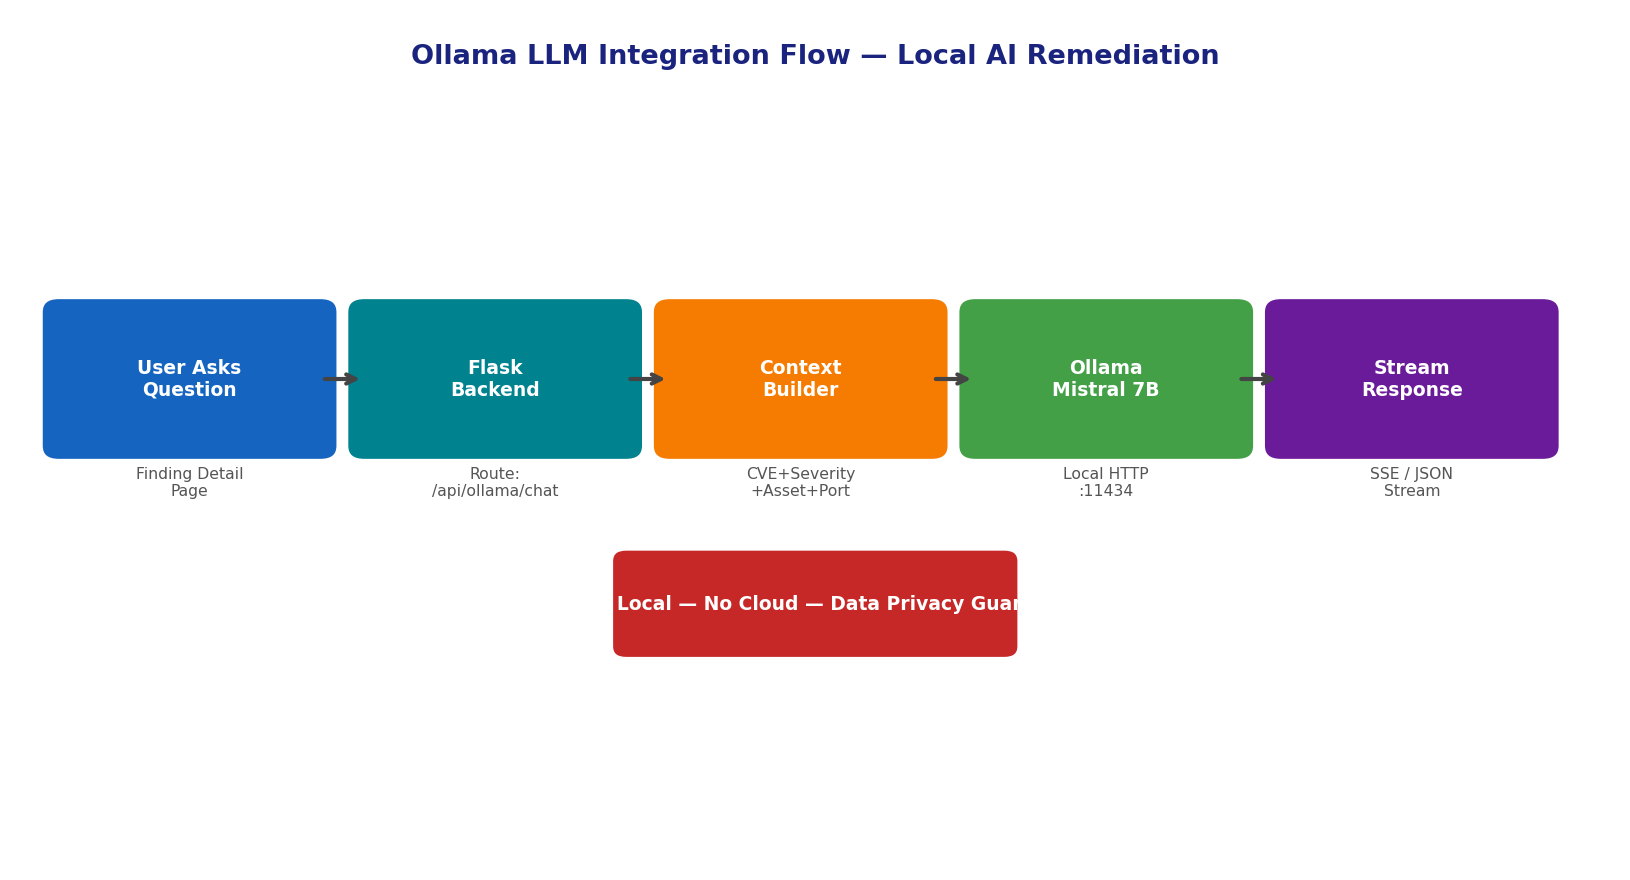
\includegraphics[width=0.92\linewidth]{img/llmflow.png}
\caption{Ollama LLM Request Flow — Local AI Remediation}
\label{fig:llmflow}
\end{figure}

The Ollama integration is the most innovative aspect of this project. The system constructs a context-rich prompt for each user question, ensuring the AI has full awareness of the specific vulnerability being discussed.

\begin{lstlisting}[style=python, caption={Ollama Service — Context-Aware Prompting}, label={lst:ollama}]
class OllamaService:
    """
    Manages communication with local Ollama instance for
    context-aware vulnerability remediation assistance.
    """
    OLLAMA_URL = "http://localhost:11434/api/chat"
    MODEL = "mistral"
    
    SYSTEM_PROMPT = """You are a Tenable vulnerability remediation expert.
When a user shares a vulnerability finding, you must:
1. Explain what the vulnerability is and why it is dangerous
2. Rate its severity and provide CVSS context
3. Provide step-by-step remediation commands appropriate for the OS
4. Suggest validation steps to confirm the fix worked
5. Recommend rollback steps if the fix causes issues
Be concise, technical, and practical. Use command blocks for CLI instructions."""

    @classmethod
    def build_context_prompt(cls, finding: Finding, user_message: str) -> list:
        """Build full conversation context including finding metadata."""
        system_context = f"""{cls.SYSTEM_PROMPT}

=== CURRENT FINDING CONTEXT ===
Finding ID:    #{finding.id}
Plugin:        {finding.plugin_id} — {finding.plugin_name}
Severity:      {finding.severity} (CVSS: {finding.cvss_score})
Asset IP:      {finding.asset.ip_address}
Asset OS:      {finding.asset.os or 'Unknown'}
Port/Protocol: {finding.port}/{finding.protocol}
CVEs:          {', '.join(finding.cve_ids or []) or 'None listed'}
Status:        {finding.status}
Due Date:      {finding.due_date.strftime('%Y-%m-%d') if finding.due_date else 'No SLA'}
Description:   {(finding.description or '')[:500]}
"""
        return [
            {"role": "system", "content": system_context},
            {"role": "user", "content": user_message}
        ]

    @classmethod
    def chat(cls, finding: Finding, user_message: str,
             history: list = None) -> str:
        """Send message to Ollama and return streamed response."""
        messages = cls.build_context_prompt(finding, user_message)
        if history:
            messages = messages[:1] + history + messages[1:]
        
        response = requests.post(
            cls.OLLAMA_URL,
            json={"model": cls.MODEL, "messages": messages, "stream": False},
            timeout=120
        )
        return response.json()["message"]["content"]
\end{lstlisting}

\subsection{SLA Engine}

The SLA engine runs as a scheduled background task, checking all non-closed findings against their due dates:

\begin{lstlisting}[style=python, caption={SLA Monitoring Service}, label={lst:slaengine}]
def check_sla_compliance():
    """
    Scheduled job: scan all active findings for SLA breaches.
    Sends OVERDUE and HALF_SLA notifications.
    """
    now = datetime.utcnow()
    
    active_statuses = ['NEW', 'ASSIGNED', 'IN_PROGRESS']
    findings = Finding.query.filter(
        Finding.status.in_(active_statuses),
        Finding.due_date.isnot(None)
    ).all()
    
    for finding in findings:
        sla = SLAPolicy.query.filter_by(severity=finding.severity).first()
        total_days = timedelta(days=sla.days_to_fix)
        elapsed = now - finding.first_seen
        
        # Check for overdue
        if now > finding.due_date:
            notify_if_not_exists(
                finding, NotificationType.OVERDUE,
                f"Finding #{finding.id} is OVERDUE by "
                f"{(now - finding.due_date).days} days"
            )
        
        # Check for half-SLA warning
        elif elapsed >= total_days * (sla.warn_at_percent / 100):
            notify_if_not_exists(
                finding, NotificationType.HALF_SLA,
                f"Finding #{finding.id} has consumed "
                f"{sla.warn_at_percent}% of its SLA window"
            )
\end{lstlisting}

\subsection{Email Notification Service}

\begin{lstlisting}[style=python, caption={Email Notification Dispatch}, label={lst:email}]
def send_notification(notification: Notification) -> bool:
    """
    Send email for a notification event and log delivery.
    """
    subject_map = {
        'ASSIGNED':                '[VMS] Finding Assigned to You',
        'OVERDUE':                 '[VMS] URGENT: Finding Overdue',
        'HALF_SLA':                '[VMS] SLA Warning — Action Required',
        'UNMAPPED_FINDINGS':       '[VMS] Unmapped Findings Detected',
        'RISK_ACCEPTANCE_REQUEST': '[VMS] Risk Acceptance Request Pending',
    }
    
    delivery = EmailDelivery(
        notification_id=notification.id,
        recipient_email=notification.recipient.email,
        subject=subject_map.get(notification.type, '[VMS] Notification'),
        status='PENDING'
    )
    db.session.add(delivery)
    
    try:
        msg = Message(
            subject=delivery.subject,
            recipients=[delivery.recipient_email],
            html=render_template(
                f'emails/{notification.type.lower()}.html',
                notification=notification
            )
        )
        mail.send(msg)
        delivery.status = 'SENT'
        delivery.sent_at = datetime.utcnow()
        db.session.commit()
        return True
    except Exception as e:
        delivery.status = 'FAILED'
        delivery.error_message = str(e)
        delivery.retry_count += 1
        db.session.commit()
        return False
\end{lstlisting}

\section{Security Architecture}

\subsection{Authentication and Authorization}

The VMS uses Flask-Login for session management with the following security measures:

\begin{itemize}
  \item \textbf{Password Hashing}: bcrypt with cost factor 12 (approximately 200ms per hash)
  \item \textbf{Session Security}: HTTPOnly and Secure cookie flags; 8-hour session expiry
  \item \textbf{CSRF Protection}: Flask-WTF CSRF tokens on all POST forms
  \item \textbf{Role Enforcement}: Custom \texttt{@role\_required} decorator on all restricted routes
\end{itemize}

\begin{lstlisting}[style=python, caption={Role-Based Access Control Decorator}, label={lst:rbac}]
from functools import wraps
from flask_login import current_user
from flask import abort

def role_required(*roles):
    """Decorator to restrict endpoint access by user role."""
    def decorator(f):
        @wraps(f)
        def decorated_function(*args, **kwargs):
            if not current_user.is_authenticated:
                return redirect(url_for('login'))
            if current_user.role not in roles:
                abort(403)
            return f(*args, **kwargs)
        return decorated_function
    return decorator

# Usage example:
@app.route('/admin/users')
@role_required('admin')
def manage_users():
    users = User.query.all()
    return render_template('admin/users.html', users=users)
\end{lstlisting}

\section{Summary}

This chapter provided a comprehensive technical blueprint of the VMS, covering: the technology stack and rationale, the three-tier architecture, all ten database tables with full SQL DDL, the state machine for finding lifecycle, the Nessus import algorithm with deduplication, the Ollama integration with context-aware prompting, the SLA monitoring engine, and the email notification system. These designs form the basis for the implementation presented in the next chapter.
